\section{历史评价协议}\label{app:history}
早期H1使用清洗后5202条记录，恢复3641训练和1561验证，与当前完整样本协议不同。LightGBM与HistGB各半融合的验证MSE为1.579267；从旧PCA表恢复的XGBoost40轮基线为1.659235。旧网络1.65340仅保留历史汇总，未找到逐条预测，不以其建立主要配对推断。

H1旧PCA表有23个成分，历史记录指出其变换在划分前拟合，且样本人群经过筛选。当前存档能恢复该表示上的部分基线数值，不等于能完整重建当时全部缩放/PCA拟合状态。故不能将其与当前29成分的探索输出混用，或把历史误差差额全部归因于取消PCA。

H2仅使用原train5642条训练，在训练CV选择HistGB350轮、7叶、叶最少40、L2=30，与LightGBM350轮、7叶、叶最少60、L2=30，各50\%；两者学习率均0.03。其A/B MSE分别1.730496/1.274190，同协议Ridge为1.792473/1.379045。表\ref{tab:historical}仅在各历史协议内部比较。
\begin{table}[htbp]
\small
\setlength{\tabcolsep}{5pt}
\centering
\caption{两套历史协议的独立结果}
\label{tab:historical}
\begin{tabular}{L{0.08\linewidth}L{0.18\linewidth}L{0.45\linewidth}L{0.17\linewidth}}
\toprule
协议 & 评价行 & 模型 & MSE \\
\midrule
H1 & 1561验证 & legacy\_linear & 1.714056 \\
H1 & 1561验证 & legacy\_xgb\_40 & 1.659235 \\
H1 & 1561验证 & LGB+HistGB各半 & 1.579267 \\
H2 & A1000 & Ridge & 1.792473 \\
H2 & A1000 & HistGB+LGB各半 & 1.730496 \\
H2 & B1000 & Ridge & 1.379045 \\
H2 & B1000 & HistGB+LGB各半 & 1.274190 \\
\bottomrule
\end{tabular}
\end{table}


H2以2017年10月20日分割4348条较早记录和1294条较晚记录作日期压力检查，模型MSE1.344691、Ridge1.389144。结构先由完整train选出，因此这不是严格无泄漏的时间外推估计；该项仅由保存JSON追溯，未找到对应逐行预测，不作为已独立重算的证据。
图\ref{fig:history}保留H1历史图示，用于说明该协议的模型对照及尾部现象，不与当前主协议直接排名。
\begin{figure}[htbp]
\centering
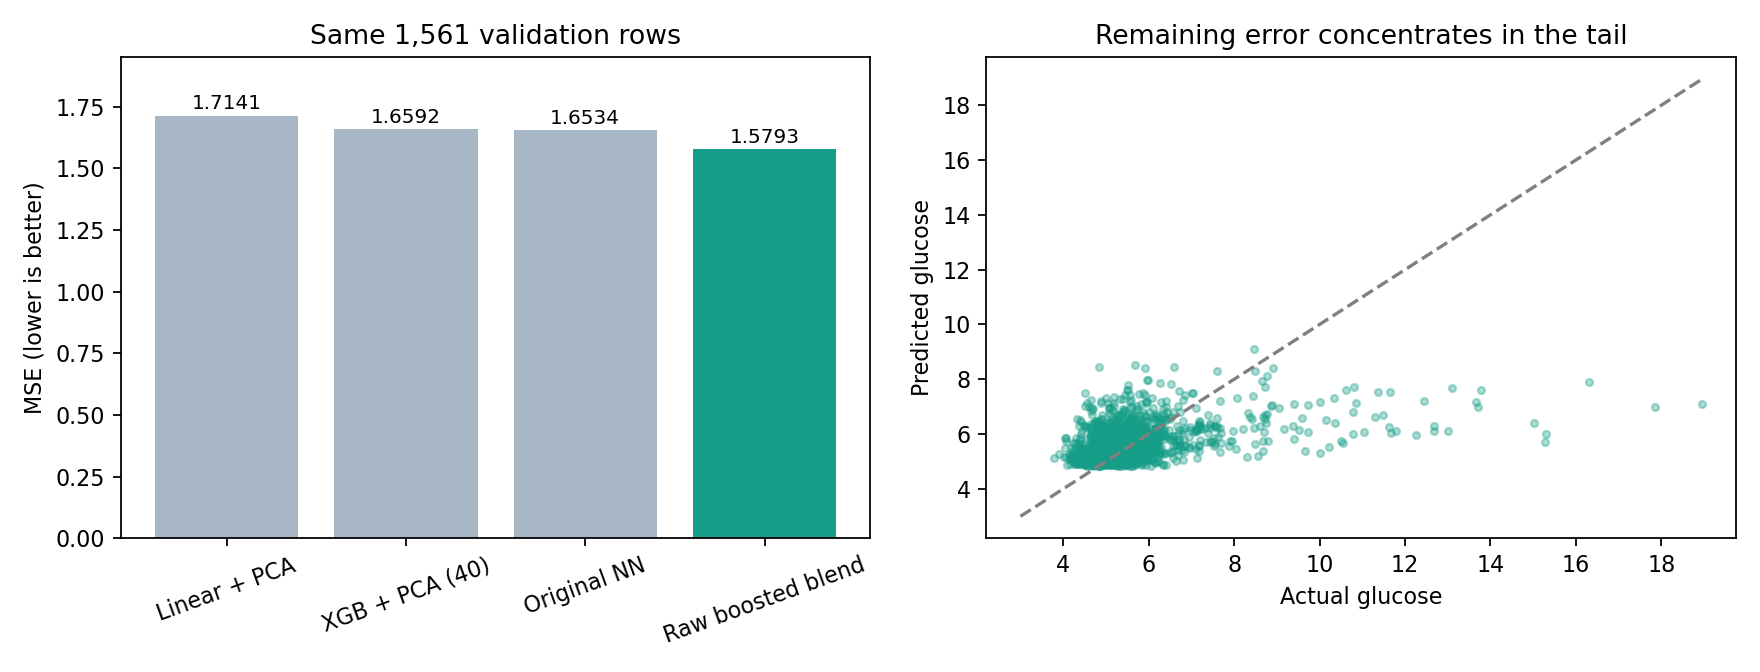
\includegraphics[width=0.94\linewidth,height=0.68\textheight,keepaspectratio]{paper/figures/paper_optimized_C004_O03.png}
\caption{历史H1的1561条验证记录对照；旧网络仅有历史汇总值，不能作为当前主协议成绩或配对推断依据。}
\label{fig:history}
\end{figure}
